% !TeX root = ../tfg.tex
% !TeX encoding = utf8

\chapter{Mathematical fundamentals of Machine Learning}\label{ch:1-MathematicalFundamentalsML}


\section{Introduction}
Machine learning is a field closely related to both computer science and statistics. It initially evolved as a sub-field of research within the broader domain of artificial intelligence. In an informal way, we can say machine learning consists of computer algorithms that generalise knowledge from patters found in data to make predictions in unknown situations, in other words: ``learning''. This is a skill that becomes natural to humans in many aspects of life throughout history. We can think from some tribes or farmers understanding of weather, all the way to doctors; all of them have acquired a level of expertise on specific fields as a result of many iterations of observing meaningful indicators and their connection to forthcoming occurrences. Additionally, this knowledge passes from generation to generation whether verbally or documented.  However, the amount of data a single human can process will always be limited since the process of learning is constrained by time, economic factors and complexity of the domains. There is where the potential of machine learning lies. This field is attractive and revolutionary because it provides us the ability to learn from extremely large data sets whose patterns tend to be very complex. Humans not only cannot handle the big dimensions of the dataset but also cannot really understand the mechanisms of the system to be able to model it with equations. Instead, machine learning assumes a general mathematical model which is then tuned to the specific problem using the provided data. The resulting model produces reliable predictions although it usually does not show the relationships present in the data that induce that behaviour or output. This is why machine learning techniques are usually conceived as a ``black box'' that is fed with data and learns to generate reliable outputs. This is one of the strengths of machine learning: its tools can be applied to a wide range of tasks and different domains. However, one of the most significant criticisms is precisely the opacity of the techniques, since it is hard to follow the decision making process of a model that is not formulated carefully to capture the essence of a mechanism as in physics or statistics. For example, data on demographic, medical and social context are quite risky  to model since we have limited understanding of the input/output process. Image classification also presents this challenge, where the objective is to assign labels to images based solely on their digital representation. Understanding what makes an image a dog or a cat proves to be a complex procedure. Nevertheless, in the context of classification, rather than understanding the intricacies of the labeling process, the goal is to replicate it.

In this introduction we have broadly mentioned that ``the model learns from data''. Next, we will dive deeper into this statement that comprises the most important components of a machine learning problem: the model, the data and the learning procedure.  We will try to understand what happens in the ``black box'' (\autoref{fig:black_box}) with a mathematical study of machine learning techniques.

\begin{figure}
    \centering
    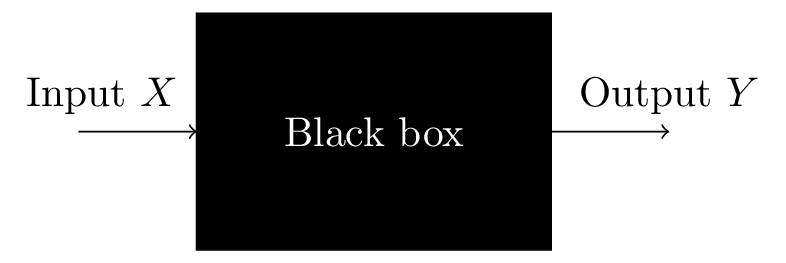
\includegraphics[width=0.5\linewidth]{img/img-ch1/black_box.png}
    \caption{Machine learning blackbox paradigm whose goal is to reproduce input/output pairs based on prior observations.}
    \label{fig:black_box}
\end{figure}


\section{Supervised learning}
First, we  will present the two fundamental learning problems that are faced in the context of machine learning: supervised and unsupervised. The problem of supervised learning can be described in the following formulation:

\begin{definicion}[Supervised learning problem]
    Let $\mathcal{X}$ be an input domain, $\mathcal{Y}$ be an output domain and $\mathcal{D} = \left\lbrace (x_1,y_1),...,(x_M,y_M)\right\rbrace \subset \mathcal{X} \times \mathcal{Y}$ be a dataset that contains inputs $x_i$ and target outputs $y_i$ sampled from a probability distribution $p(x,y)$. Given a new unclassified input $x \in \mathcal{X}$, guess or predict the corresponding output $y \in \mathcal{Y}$
\end{definicion}

In the context of unsupervised learning discussed here, the data samples lack labels, and the objective is to draw similar samples.

\begin{definicion}[Unsupervised learning problem]
    Let $\mathcal{X}$ be an input domain and $\mathcal{D}=\left\lbrace x_1, ..., x_M\right \rbrace \subset \mathcal{X}$ be a dataset of input samples drawn from a probability distribution $p(x)$. The problem consists on drawing a new sample from $p$. 
\end{definicion}

There are other tasks in unsupervised learning such as clustering and dimensionality reduction.

This thesis will be constrained to the case of supervised learning tasks. The standard procedure in supervised learning can be summarized in the following steps:
\begin{enumerate}
    \item Choose a model family $\left\lbrace f \right\rbrace$, that is, a set of trial functions that map inputs from $\mathcal{X}$ to outputs from $\mathcal{Y}$. They usually depend on a set of parameters $\theta$. Each set $\theta$ defines a particular model in the family $\left\lbrace f_{\theta}\right\rbrace$. Next we will proceed to pick the best model to reproduce the data.

    \item This task is formally known as risk minimisation. This process uses a loss function $L(f(x),y)$ which we can understand as a measure of the discrepancy between the model's prediction $f(x)$ for an input $x\in \mathcal{X}$ and its label $y \in \mathcal{Y}$. 

    \item Once we can compute the loss function, we need to choose an optimization algorithm to minimize the average loss over all the data depending on the parameters. Popular choices are gradient descent and stochastic gradient descent.
\end{enumerate}

The difficulty in machine learning lies in the task of selecting the most suitable model without having access to all the data, but instead only having a finite set of examples. Consequently, the essence of learning lies in choosing a model that generalises well from these limited examples to the entire data domain.

As we can see, the model, the data and the learning procedure (which corresponds to the last two steps) are the main components of supervised learning.

\subsection{Data}
Data is the starting point of machine learning and its fuel. The dataset of a supervised learning problem  ${\mathcal{D} = \left\lbrace (x_1,y_1),...,(x_M,y_M)\right\rbrace \subset \mathcal{X} \times \mathcal{Y}}$ is sampled from a joint distribution $p(x,y)$. The set of data samples is taken independently and identically distributed, shortened iid. This is a strong assumption that means that any sample does not depend on the value of the others and has been drawn from exactly the same distribution. This does not really correspond with real life situations but facilitates the learning theory built upon it. Learning in non-iid scenarios remains an open research question. 

We are abstractly talking about data, although what it really is? A \textbf{dataset} is a collection of \textbf{data samples}. Each data sample is a description of an event, an object or the item in question. This description is a collection of \textbf{attributes} or features and their values, which can be qualitative or quantitative, are called \textbf{attribute values}. \autoref{fig:example_dataset} depicts an example of a dataset.

Let ${\mathcal{D} = \left\lbrace (x_1,y_1),...,(x_M,y_M)\right\rbrace \subset \mathcal{X} \times \mathcal{Y}}$ be a dataset containing $M$ samples: $x_i \in \mathcal{X}$ and its corresponding label $y_i \in \mathcal{Y}$. Each data sample $x_i = (x_{i1},..., x_{iK}) \in \mathcal{X}$ is a vector of attributes in the $K$-dimensional input space $\mathcal{X}$ and $x_{ij}$ is the value of the $j$th attribute of the sample $x_i$. Regarding the output space, it determines an important distinction in the type of supervised learning problem to be solved. If $\mathcal{Y}$  is a set of discrete class labels $\left \lbrace l_1, ... l_R \right\rbrace$, we are dealing with a \textbf{classification} problem. In the particular case of $\mathcal{Y} = \left\lbrace l_1, l_2 \right\rbrace$ consits on two labels, then it is called a \textbf{binary classification} problem. If the output space is continuous, such as the space of real numbers $\mathbb{R}$ or an interval therein, then it is a \textbf{regression} problem, that is, the prediction is continuous-valued.

\begin{figure}
    \centering
    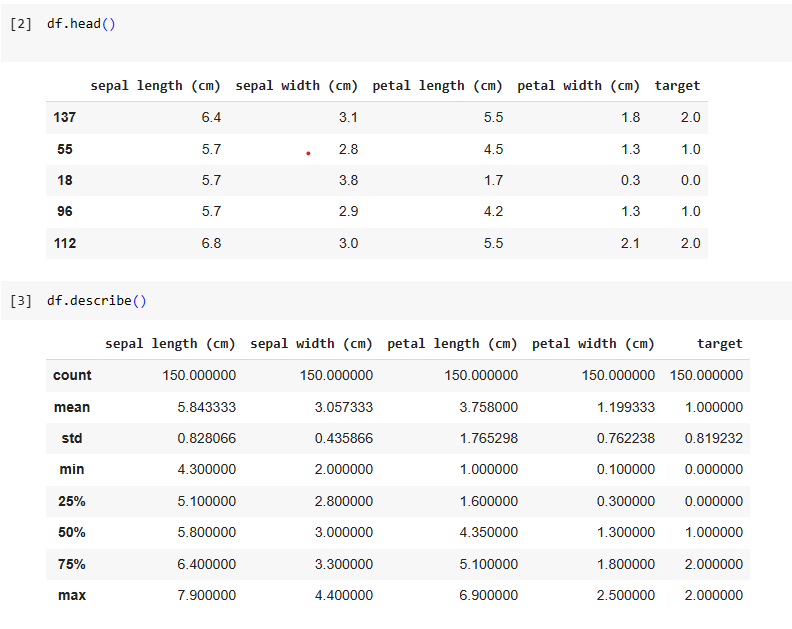
\includegraphics[width=0.8\linewidth]{img/img-ch1/iris_dataset.png}
    \caption{Example of a dataset. It corresponds to the scikit-learn Iris Dataset.\\ This data sets consists of 3 different types of irises’ (Setosa, Versicolour, and Virginica) thus, define a three label classification problem. \\
    There are four attributes: petal and sepal length and width.}
    \label{fig:example_dataset}
\end{figure}


It is desirable to have a data input space $\mathcal{X}$ in $\mathbb{R}^K$, but sometimes raw data is not from a numerical domain and it is needed to first find a suitable quantitative representation of the attributes. There are different techniques depending on the type of data, such as text or images. We cannot go into greater depth because it is a field beyond the scope of this thesis. 

There is vital step for any machine learning application: \textbf{data pre-processing}. This practice impacts the output of the machine learning algorithm and thus, improves its predictive power. Real world data is usually incomplete, dirty and inconsistent, hence data preprocessing techniques are needed to improve the accuracy and efficiency of the machine learning model used. Dirty data include missing data and wrong noisy data . The presence of a high proportion of the data is dirty, implies that the outcome of applying a machine learning algorithm will likely result in an unreliable model. So first, the data must be cleaned to remove or repair dirty data. Then, a series of data transformations are performed because the data collected in a dataset may not be useful enough, that is, the original attributes may have a meaning in its domain but are not convenient to obtain accurate predictions. There are a series of available transformations to change the original attributes or to generate new attributes with better properties. We can point out data normalization, polynomial transformations, one-hot-enconding (to transform categorical data), dimensionality reduction techniques, among others. For a more in-depth exploration of this topic, we would recommend consulting the book \cite{garcia2015data}, which provides comprehensive coverage and valuable insights on the subject of data pre-processing.

Finally, we have to mention the routinary division of the dataset into three subsets called: training, validation and test. The process of ``learning'' of the ML algorithm is also well-known as training. As we have mentioned before, learning is equivalent to generalising well. The training set is used to minimise the cost function (the average of the loss values coming from all data samples). The validation set is used to estimate the performance after training in order to adapt hyperparameters of the algorithm. The model is implicitly fitted to the validation set because we discard those models that did not perform well on this data. Once the model is fully specified, the test set is used for the final evaluation of the model's generalization ability to provide an unbiased evaluation of the final model. The separation of data into these three partitions is really important for obtaining a good model: one that can generalize well to unseen instances, avoiding overfitting. 


\subsection{Model}

The second main component of machine learning is a model, or precisely, a model family. The goal is to obtain a model that fits the data and produces reliable outputs. In mathematics, a model is a map from an input space $\mathcal{X}$ to an output space $\mathcal{Y}$, in other words, a function that reproduces the pattern in the data.
$$\mathcal{X} \longrightarrow \mathcal{Y}$$
In the context of computation, this mapping is achieved through an algorithm. At a higher level of abstraction, a model sets the hypothesis or rules that leads from input to output. Therefore, models in machine learning are functions, algorithms or rules that establish a connection between input data and output, depending on the point of view we fix. We will continue with the mathematical formulation:

\begin{definicion}[Deterministic model]
    Let $\mathcal{X}$ be an input domain and $\mathcal{Y}$ an output domain for a supervised machine learning problem. We define a deterministic model as a function 
    \begin{equation}
        f: \mathcal{X} \longrightarrow \mathcal{Y}, \quad f(x) = y,\quad x\in \mathcal{X},\, y \in \mathcal{Y}
    \end{equation}
\end{definicion}

Usually, this model depends on a set of parameters $\theta$ and hence defines a model family $\left\lbrace f_{\theta} \right\rbrace$

Depending on the output domain $\mathcal{Y}$ we can distinguish between deterministic models for regression and classification tasks.

Theoretically, machine learning methods could use any possible mapping function $$f: \mathcal{X} \longrightarrow \mathcal{Y}$$ to make predictions of a label $y\in \mathcal{Y}$ by computing $\hat{y}=f(x)$. The collection of all possible maps from the input space to the output domain is denoted by $\mathcal{Y}^{\mathcal{X}}$. To obtain the best model that fits our data, we have to search over this set $\mathcal{Y}^{\mathcal{X}}$. However, it is usually far too extensive for practical machine learning methods to fully explore it. As an example, if we consider a regression problem with dataset in which every sample is only characterized by an real-valued attribute and a real-valued label, then $\mathcal{Y}^{\mathcal{X}}$ would be the collection of all real functions of real variable. Instead, the problem would get simplified if we search for the best model in a subset of the real functions of real variable such as linear functions. In that case we are tackling a regression problem with a linear regression algorithm. In general, practical machine learning methods search and evaluate only a small subset of all possible maps $\mathcal{Y}^{\mathcal{X}}$. This subset of computationally feasible maps is what we referred as model family (denoted before as $\left\lbrace f \right \rbrace$, also called hypothesis space $\mathcal{H}$. The selection of a model family for a machine learning problem is a design choice which involves a tradeoff between computational complexity and the statistical properties of the resulting machine learning method.  This choice takes into account the computational resources at the disposal of a machine learning method. Different computational infrastructures tend to align with different hypothesis spaces. For instance, deep learning methods deployed in a cloud computing environment typically use much larger hypothesis spaces derived from deep neural networks. While deep learning methods would be an overkill for a small embedded system, which would perform much better with a linear hypothesis space. 

In a general sense, the design choice regarding the model family of a machine learning method has two main demands to be balanced: 
\begin{itemize}
    \item The model family as to be sufficiently large so that it contains at least one accurate predictor map $\hat{f}\in \left\lbrace f \right\rbrace$. If the model family is too small, it may not encompass a predictive mapping necessary to capture the (potentially complex and nonlinear) relationship between inputs and outputs.

    \item It has to be sufficiently small such that its processing fits the available computational resources including memory, bandwidth and processing time. At the same time, we must be able to search efficiently to find a good model. Constraining the size of the hypothesis space is also related to the prevention of overfitting since in a large model family we might, by chance, stumble upon a function that almost perfectly predicts the labels of the training set while showing poor generalization power for other data.
\end{itemize}


\subsection{Learning procedure}

A machine learning method has to select the best model from the model family of all computationally feasible predictor maps. This raises the question: which model is the best model out all the possible ones? We need a measure of quality of a model, that is, how close are the model predictions to the target labels. There is where the concept of \textbf{loss function} appears. 

\begin{definicion}[Loss function]
    A loss function is a map
    \begin{align}
        L: \mathcal{X} \times \mathcal{Y} \times \mathcal{H} &\longrightarrow \mathbb{R}^{+} \\
        ((x,y),f) &\longmapsto L(f(x),y)
    \end{align}
    which assigns a pair consisting of a input $x \in \mathcal{X}$, its label $y\in \mathcal{Y}$ and a model $f$ to the non-negative real value $L(f(x),y)$ named loss value.
\end{definicion}

The loss value $L(f(x),y)$ measures the difference between the true label $y $ and the prediction by the model $f(x)$. Now that we have formulated this concept, we can rephrase the basic procedure of machine learning to find a model out of all the model family that minimizes the loss $L(f(x),y)$ for all data inputs.

The loss function is another design choice for the machine learning technique. This decision should take into account the computational complexity for finding a minimum loss (benefiting differentiable and convex functions), robustness to outliers, statistical aspects and interpretability. There exist numerous loss functions, and perhaps the simplest one for classification tasks relies on a model's accuracy, which measures the proportion of correctly classified examples:
\begin{equation}
    \text{accuracy} = \frac{\text{number of samples classified correctly}}{\text{total number of samples}}
\end{equation}
The corresponding loss would be the error:
$$\text{error} = 1-\text{accuracy}$$

Most machine learning methods use a continuous-valued loss function, since differentiability is desirable to compute gradients. One of the most popular loss functions is the norm in $l_2$ or squared Euclidean distance which is known as \textbf{mean-squared-error loss}
$$L(f(x),y)=(f(x)-y)^2$$
The norm in $l_1$ also provides us another loss function:
$$L(f(x),y)=|f(x)-y|$$
Other options are the \textit{hinge loss}
$$L(f(x),y) = \max (0, 1-yf(x))$$
and the \textit{logistic loss}
$$L(f(x),y) =\log (1+e^{yf(x)})$$

The loss function is the starting point of the \textbf{risk minimisation} process that consists on minimising the expected or average loss (called risk ) of a model over the data distribution.
\begin{definicion}[Risk]
    Let the inputs $x \in \mathcal{X}$ and outputs $y \in \mathcal{Y}$ to a supervised learning problem be sampled from a distribution $p(x,y)$. The \textbf{expected loss} or \textbf{risk} of a model $f$ with loss $L$ is defined as
    \begin{equation}
        \mathcal{R}_f = \mathbb{E}[L_f] = \int_{\mathcal{X}\times \mathcal{Y}} L(f(x),y) p(x,y) dx\, dy
    \end{equation}
    Note that the integral runs over all possible data pairs and thus, the expectation is taken over the data distribution.
\end{definicion}

The risk provides an indication of the model's performance across the entire data domain, with a lower risk indicating better performance. The goal to solve a supervised learning problem will be to minimise the risk, although the integral over all possible data pairs is impossible to compute in practice, so we need to estimate the risk over the $M$ data samples we are provided in a dataset. This estimation is called \textbf{empirical risk}.
\begin{definicion}[Empirical risk]
    Consider the dataset ${\mathcal{D} = \left\lbrace (x_1,y_1),...,(x_M,y_M)\right\rbrace \subset \mathcal{X} \times \mathcal{Y}}$. The empirical risk estimates the risk over the dataset as the average loss:
    \begin{equation}
        \hat{\mathcal{R}}_f = \hat{\mathbb{E}}[L_f] = \frac{1}{M}\sum_{i=1}^M L(f(x_i), y_i)
    \end{equation}
\end{definicion}

This estimation is warranted because of the law of large numbers, departing from the assumption that we consider the dataset to be independent and identically distributed variables from the distribution $p(x,y)$. Therefore, the sample average converges to the expected value if the number of samples $M$ of the dataset $\mathcal{D}$ is sufficiently large. 

In practice, we select a model out of the model family minimising the empirical risk on the given dataset, that is, finding the model $f^*$ such that $$f^* = \min_{f \in \mathcal{H}} \hat{\mathcal{R}}_f$$
In parametrised model families, model selection translates to optimising the parameters. Therefore, the empirical risk minimisation can be reformulated as finding the parameter $\theta^*$ such that
$$\theta^*=\min_{\theta} \hat{\mathcal{R}}_{f_{\theta}}$$

Machine learning should solve the empirical risk minimisation problem without overfitting: there is an optimal solution of the empirical risk over the training data that performs poorly on new data. There are different strategies to prevent the model from overfitting: \textbf{regularisation techniques}. The most common one is to add a regularisation term $g(f_{\theta})$ to the empirical risk and minimise the cost function
$$C(\theta)=\hat{\mathcal{R}}_{f_{\theta}} + g(f_{\theta})$$
These regularisation terms penalize the model and impose additional constraints, for example the $l_1$ regulariser
$$g_{l_1}(\theta)=\sum_{i}|\theta_i|$$
benefits parameters with a small absolute value, while the $l_2$ regularisation term
$$g_{l_2}(\theta)=\sum_i \theta_i^2$$
adds preference to parameters with a small $l_2$ norm.

Once we have formulated the cost function, the learning procedure consists on an optimisation problem. While there is an extensive theory and algorithms for convex optimisation problems,  machine learning tasks usually fall into non-convex optimisation problems for which there is significantly less information available. The popular choice to tackle this sort of non-convex optimisation are iterative searches that progressively calculate better candidates for the parameters of a model.
In situations where there are multiple parameters and optimization occurs within high-dimensional spaces, we need to understand the landscape of the cost function. The main source of information in such cases is gradients: a vector of partial derivatives of a function with respect to its inputs. The gradient provides the direction of the most significant incline in the cost landscape.

\textbf{Gradient descent} is an iterative algorithm for finding the minimum of a differentiable function. The general idea of this algorithm is to update the parameters $\theta$ of a cost function $C(\theta)$ iteratively towards the direction of steepest descent in order to minimize a cost function. We can think of this situation in a real world scenario: suppose you are lost in the mountains blindfolded, you can only feel the slope of the ground below your feet. Your goal is to reach to the lowest point going downhill in the direction of the steepest slope. 

This is mathematically expressed as
$$\theta_{t+1} = \theta_{t}-\eta\nabla C(\theta_t)$$
where $\eta$ is a parameter called learning rate that determines the step size at each iteration and $t$ is an integer that corresponds to the current iteration. \autoref{fig:gradient_descent} illustrates this algorithm for a really simple scenario.

If the learning rate is too small, the algorithm will have to perform many iterations to converge. Whereas if the learning rate is too high, you might jump across the valley and end up on the other side, perhaps even at a higher point than in the previous step and eventually the algorithm may diverge. This situations are depicted in \autoref{fig:learning_rates}.

\begin{figure}
    \centering
    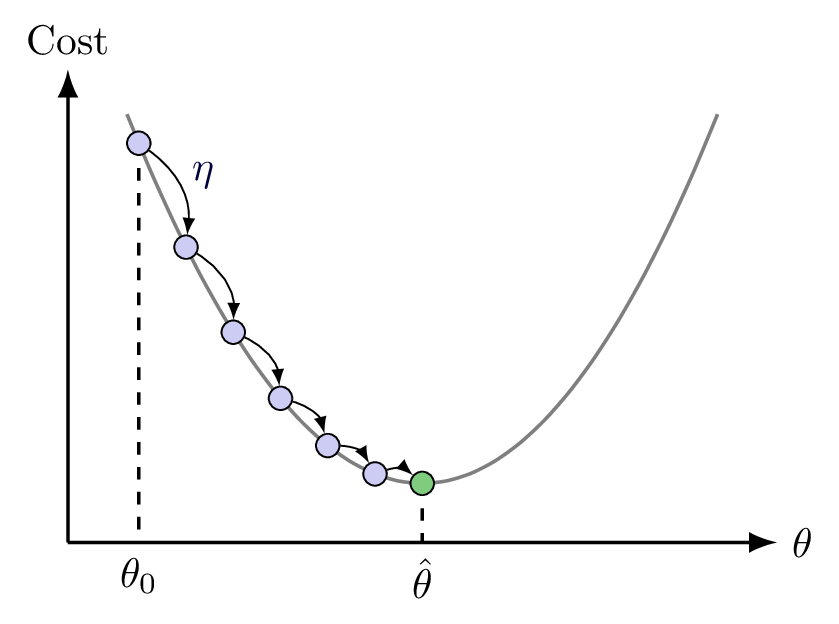
\includegraphics[width=0.6\linewidth]{img/img-ch1/gd.png}
    \caption{Gradient descent}
    \label{fig:gradient_descent}
\end{figure}

\begin{figure}
    \centering
    \begin{subfigure}{0.5\textwidth}
        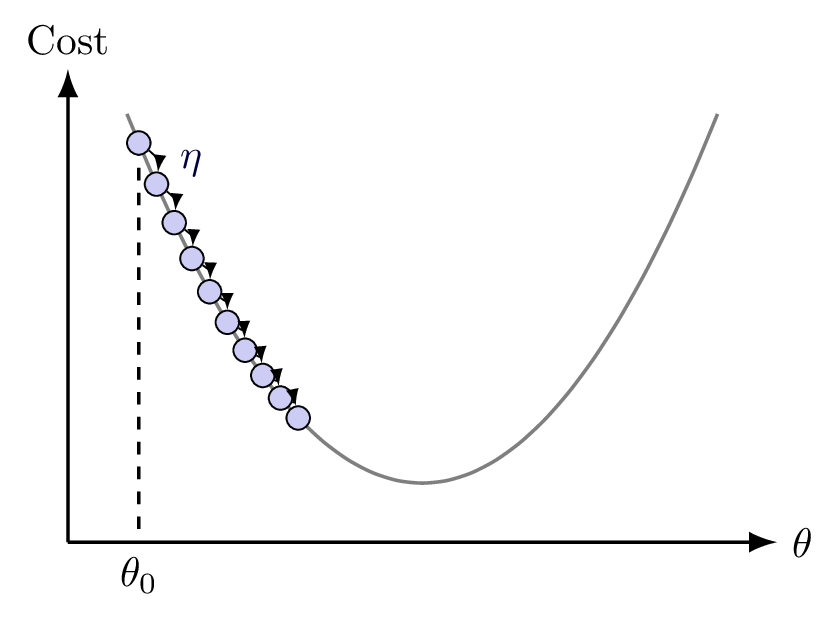
\includegraphics[width=\linewidth, keepaspectratio]{img/img-ch1/gd_small.png} 
        \caption{Gradient descent algorithm taking a $\eta$ learning rate too small}
        \label{fig:GD small learning rate}
    \end{subfigure}
    
    \begin{subfigure}{0.5\textwidth}
        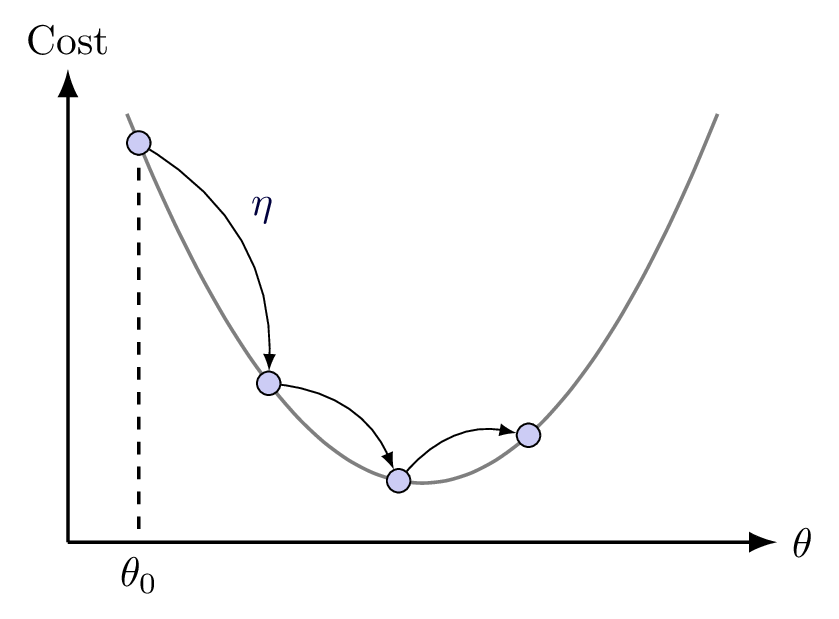
\includegraphics[width=\linewidth, keepaspectratio]{img/img-ch1/gd_big.png}
        \caption{Too big $\eta$ learning rate for gradient descent}
        \label{fig:GD big learning rate}
    \end{subfigure}
    
    \caption{Effect of different learning rates for gradient descent algorithm}
    \label{fig:learning_rates}
\end{figure}

The formula above of the gradient descent algorithm performs the purpose of the process: the gradient $\nabla C(\theta_t)$ always points towards the ascending direction in the landscape of the cost function $C$, thus $- \nabla C(\theta_t)$ points to the opposite direction, that is, the descending direction. The initial set of parameters $\theta_0$ is randomly initialized. Then, it is gradually improved, at each step attempting to decrease the cost function. 

In real case scenarios, cost functions may differ very much from the previous illustrations. There may be holes, plateaus, ridges and all sorts of irregular terrains, making convergence to the minimum very difficult.

There are several variations of the gradient descent algorithm such as batch gradient descent, stochastic gradient descent and mini-batch gradient descent. \cite{geron2022hands}

\subsection{Evaluation metrics}
After training and finding a model that performs sufficiently well, it is time to evaluate the final model on the test set. First, we need to apply the model to the test set to obtain the predictions. Then, having the predictions and the labels we can apply different metrics to evaluate the performance of the model.

There are many performance measures available. In the context of classification, we will consider the following ones:

\begin{itemize}
    \item \textbf{Accuracy.} This metric represents the ratio of correct predictions to the total number of samples.
    \begin{equation}
        \text{accuracy} = \frac{\text{number of samples classified correctly}}{\text{total number of samples}}
    \end{equation}

    It gives us a general idea of the classification power of our model, although we have to take into account that it is not a good metric in the case of a dataset with unbalanced classes since it is ``blind'' to different classes. To understand it, let's consider a dataset with 100 samples, 97 of them are labeled 0 and 3 correspond to label 1. If our model predicts label 0 for all samples, the accuracy would be of 97\% which does not represent the actual lack of classification power of the model. 
    
    \item \textbf{Confusion matrix.} 
    A confusion matrix is a table used to evaluate the performance of an algorithm. Each row corresponds to a label and each column represents a predicted label. Therefore, if $n$ is the number of labels of the dataset, the confusion matrix is a $n \times n$ table that shows the correct and incorrect predictions made by the model compared with the actual labels.

    In the case of a binary classification problem we have the following confusion matrix, considering \textit{P} is the number of positive labels (1) and \textit{N} is the number of negative labels (0). 

    
    
    \begin{table}
        \centering
        \setlength{\tabcolsep}{10pt} % Default value: 6pt
        \renewcommand{\arraystretch}{1.5} % Default value: 1
        \begin{tabular}{|c|cc|}
            \hline
             & PP  & PN \\
             \hline
            P & TP & FN\\
            N & FP & TN\\
            \hline
        \end{tabular}
        \caption{Confusion matrix of a binary classification problem.}
        \label{tab:confussion_matrix}
    \end{table}
    In figure \autoref{tab:confussion_matrix}, TP stands for true positive, FP - false positive, TN - true negative and FN - false negative. These values are used to compute other metrics.
    
    \item \textbf{Precision.} It is the ability of a model not to label as positive a sample that is negative. 
    \begin{equation}
        \text{Precision} = \frac{TP}{TP + FP}
    \end{equation}
    It is useful for unbalanced datesets, since the precision is inversely proportional to the number of false positives.
    
    \item \textbf{Recall.} It is the ability of the classifier to find all the positive samples.
    \begin{equation}
        \text{Recall} = \frac{TP}{TP + FN}
    \end{equation}
    
    \item \textbf{$F_1$ score.} It can be interpreted as the harmonic mean of the precision and recall. 
    \begin{equation}
        F_1 = \frac{2 \cdot \text{precision} \cdot \text{recall}}{\text{precision} + \text{recall}} = \frac{2 TP}{2 TP + FP + FN}
    \end{equation}
    This metrics takes values in the interval $\interval{0}{1}$. The higher $F_1$, the better is the performance of the model.
    
    
    \item \textbf{ROC curve.} It stands for Receiver operating characteristic curve. It is a graph that shows the performance of a binary classifier as its discrimination threshold (the threshold for deciding whether a prediction is labeled positive or negative) is varied. It represents the tradeoff between the TPR = true positive rate (fraction of true positives out of all the positives) and the FPR = false positive rate (fraction of false positives out of all the negatives). A perfect model would have high value of true positive rate and low value of false positive rate.

    \item \textbf{AUC.} It computes the area under the ROC curve. This metric summarizes the curve information in one number. AUC has a range of [0,1]. The greater the value, the better is the performance of our model.
\end{itemize}


Up to this point, we have observed that the objective in machine learning is to choose a model that reduces a specific cost function which depends on data samples of a particular task, with the ultimate goal of minimizing the cost when applied to unseen data. If the model is parametrised, the selection process involves optimizing or "training" these parameters minimise the cost. 

There are many methods in machine learning, that is, model function families that can be used for prediction and a training strategy for how to use the data to construct a specific model that generalises from it. In the following sections, we will introduce two classical machine learning methods: support vector machines and neural networks, that will become important in the context of quantum machine learning in the following chapters. 


\section{Support vector machines}

 Support vector machine (SVM) is a supervised learning algorithm for binary classification. In particular, SVM are one of the most well-known kernel methods. Kernel methods work out machine learning problems based on the concept of measuring similarity between data points. This similarity measure is expressed by a \textbf{kernel}.
 

 \subsection{Kernel methods}\label{subs:kernel-methods}
 \begin{definicion}[Kernel]
     Given a data domain $\mathcal{X}$, a kernel is a positive semi-definite bivariate function $\kappa : \mathcal{X} \times \mathcal{X} \longrightarrow \mathbb{R}. $ 
 \end{definicion}
 
 Mercer's theorem provides the following useful characterization of kernels.
 \begin{teorema}
     The function $\kappa: \mathcal{X} \times \mathcal{X} \longrightarrow \mathbb{R}$ is a Mercer kernel function (also known as kernel function) where:
     \begin{enumerate}
         \item it is symmetric: $\kappa (x,y) = \kappa(y,x), \, \forall x,y \in \mathcal{X}$,
         \item its kernel matrix, that is, the kernel applied on a set of data points of the input space $\mathcal{D}=\left \lbrace x_1,...,x_M\right\rbrace $ forms a $M \times M$ Gram matrix: $\mathcal{K}(i,j)=\kappa(x_i, x_j), \quad \forall i,j \in \left\lbrace1,...,n\right\rbrace$ is positive semi-definite.
     \end{enumerate}     
 \end{teorema}

 
 A great part of the theory of kernel methods relies on \textbf{``the kernel trick''}: the fact that kernel functions can be represented as inner products of data that has been mapped from its original space $\mathbb{R}^n$ into a higher dimensional space $\mathbb{R}^N$ ($n<N$), in which machine learning algorithms can solve problems by the use of inner product. This higher dimensional space receives the name of feature space $\mathcal{F}$. The potential of this idea is that in a suitable feature space we would obtain linearly separable data by a hyperplane. The function that takes original data inputs into the feature space is called \textbf{feature map} $\phi : \mathcal{X} \longrightarrow \mathcal{F} $.

 Thus, we just need to compute: 
 \begin{equation}
     \kappa(x, y) = \left< \phi(x), \phi(y) \right>_{\mathcal{F}}
 \end{equation}

 In turn, a model is expressed in terms of a kernel function. We obtain different models by replacing the kernel functions. 

Support vector machine provides a decision boundary (a hyperplane in the feature space) separating the considered classes such that its distance to each class is as large as possible. This idea derives from their initial introduction as maximum-margin classifiers, which advocates that during training, the goal is to maximize the separation between the decision boundary of a classifier and the training data points.

An introduction to maximum-margin classifiers will help us to understand better the working principle of support vector machines.

Let's consider a binary classification problem with an input domain $\mathcal{X} = \mathbb{R}^n$ and output domain $\mathcal{Y}=\left\lbrace -1, 1\right\rbrace$. 

We assume that our data is linearly separable by a hyperplane, which means that there is a normal vector $\vec{w} \in \mathbb{R}^n$ and some constants $b \in \mathbb{R}$ which define a hyperplane $\vec{w}\cdot \vec{x} +b =0$ that separates the training data so that points of the two different classes are on either side of the hyperplane. We will denote this hyperplane as $H$. We can determine to which side of the hyperplane our data $x \in \mathcal{X}$ is in terms of the sign of $\vec{w}\cdot \vec{x} +b$. 

We take a linear model as this hyperplane and simplify the vectorial notation
$$f_{w}(x) = w^T x + b$$

Linear separation can be expressed by the restriction $f_w(x_i) >0$ for data points labeled $y_i = 1$, and $f_w(x_i)<0$ for inputs of class $y_i=-1$. According to this, linear separation can be summarised in the following condition 
$$f_w(x_i)y_i > 0 \quad \forall i=1,...,M$$

There are infinite number of separating hyperplanes, but we are looking for the one that would maximize the distance to the training datapoints and therefore, obtain a classifier with a low risk because we expect unseen data to follow a similar distribution to the one that we have seen in the training data, that is, new samples of one class will be close to training samples of that class. Support vector machine looks for the separating hyperplane that maximises the distance between the closest training points and itself. This distance is known as \textit{margin}.

Let's consider $p_0$ the closest data point to $H$ and consider the hyperplane parallel to $H$ that contains $p_0$. This hyperplane and its reflection define the margin of $H$ and can be represented by the equations $\vec{w}\cdot \vec{x} +b =\pm C$ for some constant $C$. We can divide the expression by $C$ to obtain the margin hyperplanes: $$\hat{w} \vec{x} + \hat{b} = \pm 1$$
where $\hat{w}=\vec{w}/C$ and $\hat{b}=b/C$.

The separating hyperplane $H$ can be represented by $$\hat{w} \vec{x} + \hat{b} = 0$$
We will denote the margin hyperplanes as $H_1$ and $H_{-1}$ accordingly.

We are working under the assumption that there are no points inside the margin. Studying the sign of $\hat{w} \vec{x_0} + \hat{b}$ for $x_0 \in \mathbb{R}^n$ we can determine to which region it belongs:
\begin{itemize}
    \item If $\hat{w} \vec{x_0} + \hat{b} = 0$, then $x_0$ is in the hyperplane $H$.
    \item If $0<\hat{w} \vec{x_0} + \hat{b}<1$, then $x_0$ is in the margin between the hyperplanes $H$ and $H_1$.
    \item If $-1<\hat{w} \vec{x_0} + \hat{b}<0$, then $x_0$ is in the margin between the hyperplanes $H$ and $H_{-1}$.
    \item If $\hat{w} \vec{x} + \hat{b} = \pm 1$, then $x_0$ is in one the hyperplanes that defines the margin, $H_1$ or $H_{-1} $ respectively.
\end{itemize}

The condition of linear separation with margin can be expressed with the constraint:
$$f_w(x_i)y_i>1 \quad \forall i=1,...,M$$

Let's remember that our goal is to maximize the margin while preserving the condition of linear separation with margin that we have derived above. Now we will deduce what is the expression of the margin, which is the distance between the hyperplanes $H_1$ and $H_{-1}$. 

First we will see what is the distance between $H$ and $H_1$: the length of the only vector in the direction normal to $H_0$ that connects $p \in H_0$ to a point in $H_1$. Since $\hat{w}$ is normal to $H_0$, the desired vector needs to be $\alpha \hat{w}$ for some scalar $\alpha$. Therefore, $p + \alpha \hat{w} \in H_1$ and it must fulfill its equation:
\begin{align}
    \hat{w}(p+\alpha \hat{w}) +b &= 1 \\
    \hat{w}p + b + \alpha ||\hat{w}||^2 &= 1
\end{align}
Since $p \in H_0$, we have that $\hat{w}p + b =0$. We can obtain the scalar $\alpha$ from the expression above
$$\alpha ||\hat{w}||^2=1 \Longleftrightarrow \alpha = \frac{1}{||\hat{w}||^2} $$

The length of $\alpha \hat{w}$ would be $$||\alpha \hat{w}|| = |\alpha| \cdot ||\hat{w}|| = \frac{1}{||\hat{w}||^2} ||\hat{w}|| = \frac{1}{||\hat{w}||}$$

Therefore, the distance between $H_1$ and $H_{-1}$ is by symmetry the double of the distance between $H$ and $H_1$, that is $\frac{2}{||\hat{w}||}$. 

The problem of finding a hyperplane that separating the data maximizes the margin can be posed as the following optimization problem
\begin{align}
    \text{Maximize: \quad } &\frac{2}{||\hat{w}||} \\
    \text{subject to: \quad } &f_w(x_i)y_i>1 \quad \forall i=1,...,M
\end{align}

The above optimisation problem of finding the maximum margin becomes equivalent to the next minimization problem
\begin{align}
    \text{Minimize: \quad } &||\hat{w}|| \\
    \text{subject to: \quad } &f_w(x_i)y_i>1 \quad \forall i=1,...,M
\end{align}

Alternatively, it is possible to minimise $\frac{1}{2} ||\hat{w}||^2$ under the same constraint, leading to the same solution but easier to solve. Now we are going to briefly present the dual SVM problem which is equivalent to 
\begin{align}
    \text{Minimize: \quad } &\frac{1}{2}||\hat{w}||^2 \\
    \text{subject to: \quad } &f_w(x_i)y_i>1 \quad \forall i=1,...,M
\end{align}
This is a quadratic optimization problem with $n+1$ variables ($\hat{w}\in\mathbb{R}^n$ and $b\in \mathbb{R}$) and $M$ constraints. It is computationally difficult to solve when $n$ is large. The dual problem will also be a quadratic optimization problem but with $M$ variables and $M+1$ constraints. The solution gives us the same optimal hyperplane but the dual problem is often easier and it also allows us to exploit the kernel trick that we mentioned before. 

The first task is to construct the Lagrangian. The optimization variables are $b$ and $w$. There are $M$ constraints, so we introduce $M$ penalty terms and a Lagrange multiplier $\alpha_m$ for each of them. The Lagrangian is:
\begin{align}
    \mathcal{L}(b,w,\alpha) &= \frac{1}{2}w^2 +\sum_{m=1}^M \alpha_m(1- y_m(w^T x_m +b)) \\
    &= \frac{1}{2}w^2 - \sum_{m=1}^M \alpha_m y_m w^T x_m - b \sum_{m=1}^M \alpha_m y_m + \sum_{m=1}^M \alpha_m
\end{align}
First, we have to minimize $\mathcal{L}$ with respect to $b$ and $w$. We obtain its partial derivatives:
\begin{itemize}
    \item The partial derivative with respect to $b$ is the coefficient of $b$ because it appears linearly in the Lagrangian. $$\frac{\partial \mathcal{L}}{\partial b} = -\sum_{m=1}^M \alpha_m y_m$$
    \item Using some linear algebra identities, we can obtain that the gradient with respect to $w$ is 
    $$\frac{\partial \mathcal{L}}{\partial w} = w - \sum_{m=1}^M \alpha_m y_m x_m$$
\end{itemize}

We can derive the dual form by noting that the gradient of $\mathcal{L}$ with respect to $w$ is zero if 
$$w = \sum_{m=1}^M \alpha_m y_m x_m$$
On the other hand, the partial derivative with respect to $b$ is zero if $$\sum_{m=1}^M \alpha_m y_m = 0$$

Therefore, 
$$\mathcal{L}(b,w,\alpha) = \frac{1}{2}w^2 - \sum_{m=1}^M \alpha_m y_m w^T x_m  + \sum_{m=1}^M \alpha_m$$

We can substitute $w = \sum_{m=1}^M \alpha_m y_m x_m $ in the first two terms of the sum. After groping and operating we would obtain the final expression of the Lagrangian that only depends on $\alpha$
\begin{equation}
    \mathcal{L} = \sum_{m=1}^M \alpha_m - \frac{1}{2} \sum_{m,n = 1}^M y_m y_n \alpha_m \alpha_n x_m^T x_n
\end{equation}
This is know as the dual Lagrangian function. It describes a convex optimisation problem with $M$ variables, where $M$ is the number of training samples.

Once obtained this formulation, the optimisation problem is translated into an equivalent minimization task:
\begin{align}
    \text{Minimize: \quad } &\sum_{m=1}^M \alpha_m - \frac{1}{2} \sum_{m,n = 1}^M y_m y_n \alpha_m \alpha_n x_m^T x_n \\
    \text{subject to: \quad } &\sum_{m=1}^M \alpha_m y_m = 0 \\
    &\alpha_m \geq 0 \quad m=1,...,M
\end{align}

Once the optimal Lagrangian multipliers $\alpha^*$ are found, we are just missing to compute the optimal hyperplane. The optimal weights $w_*$ are obtained from the condition 
$$w_* = \sum_{m=1}^M \alpha_m^* y_m x_m$$

We can compute predictions with the linear model 
$$f_{w_*}(x) = w_*^T x + b$$
or in the dual space
$$f(x) = \sum_{m=1}^M \alpha_m^* y_m x_m^T x +b$$

It is worth noting that the dual Lagrangian optimisation expression and the model in the dual space above rely only on the inner product $\braket{x_i,x_j }$ between data samples $x_i, x_j$. We can replace this inner product with an inner product in a feature space $\mathcal{F}$ and there is where kernels appear: $\kappa(x_i,x_j)=\braket{\Phi(x_i),\Phi(x_j)}_{\mathcal{F}}$ 

This way, the linear model is turned into a linear model in the feature space:
$$f_w(x) = \braket{w, \Phi(x)}_{\mathcal{F}} + b$$
with $w \in \mathcal{F}$.

The initial condition of linear separability of the data is translated to a feature space of higher dimension. Nonlinear data can be linearly separable in a feature space where the maximum-margin classifier becomes a kernel method that can candle non separable data. This way, SVM can find nonlinear decision boundaries in input space. 


\section{Neural networks}

Artificial neural networks are a fundamental component of artificial intelligence, that has revolutionized the field of machine learning and continue to drive innovation in various domains. These computational models were born taking the brain's architecture as inspiration. The human nervous system contains cells, which receive the name of neurons. They are composed of a cell body called ``soma'' containing the nucleus and most of the cell's complex components, and many branching extensions called ``dendrites'' plus one long extension called the ``axon''. At the tip of the ramifications of the axon there are tiny structures called ``synaptic terminals'', or simply ``synapses'', which are connected to the dendrites of other neurons. \autoref{fig:bio-neuron} is an illustration of a neuron and its parts.

Biological neurons receive signals, short electrical impulses from other neurons through the synapses. A neuron fires its own signals once the incoming signal surpasses a certain threshold value. This is know as the \textbf{integrate and fire} principle, one of the simplest models of a neuron’s electrical properties and probably the most commonly used in the field of neuroscience. The strengths of synaptic connections often change in response to external stimuli. At first glance, it looks like individual neurons behave in a rather simple way, yet they are organized in a vast network comprising billions of neurons, with each neuron usually connected to thousands of other neurons. The cortex of different species has been observed to display a laminar or layered structure. Each individual layer within the cortex showcases a unique distribution of different types of neurons and their respective connections. The structure of biological neural networks remains a topic of ongoing investigation and research.

\begin{figure}
    \centering
    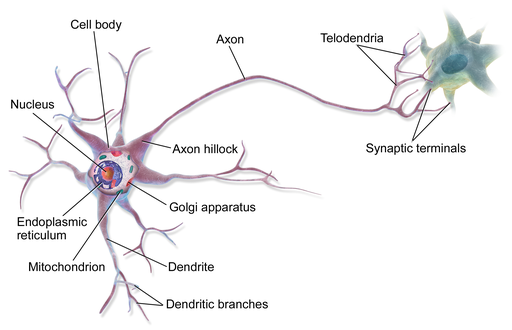
\includegraphics[width=0.7\linewidth]{img/img-ch1/Blausen_0657_MultipolarNeuron.png}
    \caption{Biological neuron. Image by BruceBlaus, \href{https://creativecommons.org/licenses/by/3.0}{CC BY 3.0}, via Wikimedia Commons}
    \label{fig:bio-neuron}
\end{figure}


This biological mechanism is simulated in artificial neural networks. The artificial neurons are the computational units that are connected with each other through weights, which model the strengths of synaptic connections present in the biological case. Every input received by a neuron is scaled by a weight factor, influencing the function computed by that specific unit. An artificial neural network processes the input values by propagating their computed values from the input neurons to the output neuron(s) while leveraging the weights as intermediary parameters, in order to learn. Similar to how biological organisms require external stimuli for learning, artificial neural networks rely on training data containing examples of input-output pairs, which serve as the external stimulus for the learning process. 

Throughout this section, we will use the term neural networks to refer to artificial neural networks, leaving behind the biological ones.

\subsection{Perceptron}
The perceptron is the simplest neural network, proposed in 1957 by Frank Rosenblatt \cite{rosenblatt1958perceptron}. It has a single input layer and an output node. It computes a weighted sum of its inputs $\left\lbrace x_1,...,x_n\right\rbrace$: $z = w_1x_1+...w_nx_n = w^T x$, where $x=(x_1,...,x_n)$ is the input vector and $w = (w_1,...,w_n)$ is the weight vector. Then, applies a non linear function $\varphi$ called the activation function. \autoref{fig:perceptron} displays the graphical representation of a perceptron.

In the original proposal of the perceptron, it was formulated with the Heaviside function, also known as step function, which is applied to that sum. Finally, it outputs the result. The model function of the perceptron is given by
\begin{equation}
    f(x,w)=H(w^T x)
\end{equation}
where $H$ is the Heaviside function (plotted in \autoref{fig:heaviside})
\begin{equation}
    H(x) =
    \begin{cases}
    0 & \text{if } z < 0 \\
    1 & \text{if } z \geq 0
    \end{cases}
\end{equation}

\begin{figure}
    \centering
    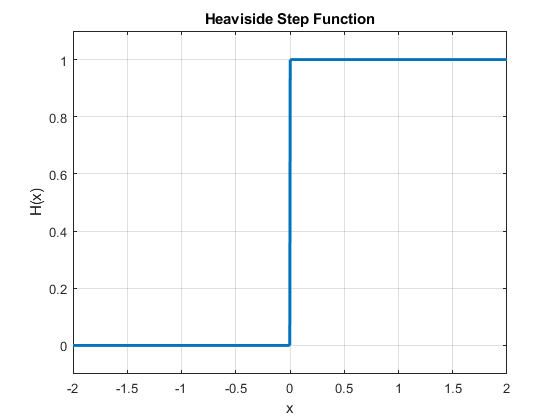
\includegraphics[width=0.7\linewidth]{img/img-ch1/heaviside_graph.png}
    \caption{Plot of the Heaviside step function}
    \label{fig:heaviside}
\end{figure}

\begin{figure}
    \centering
    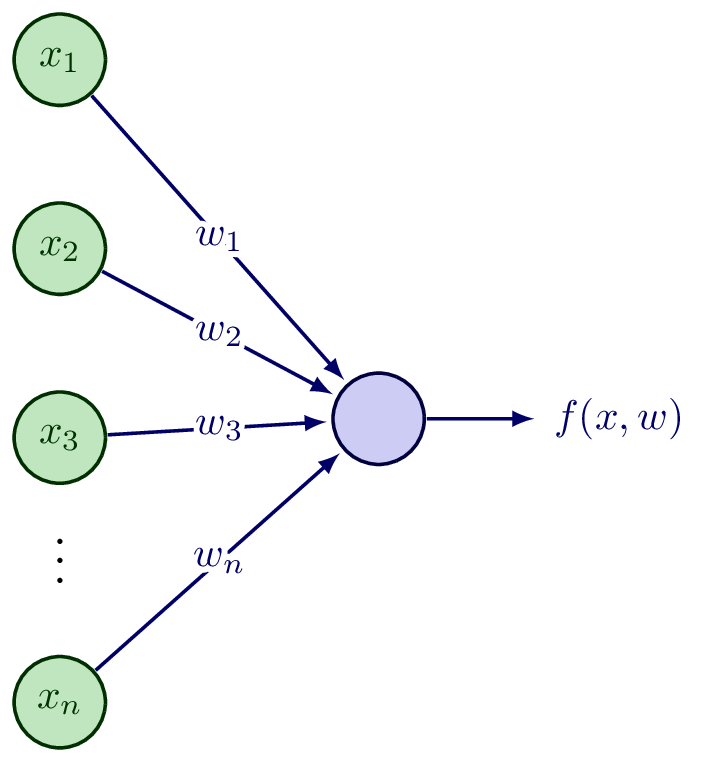
\includegraphics[width=0.5\linewidth]{img/img-ch1/perceptron.png}
    \caption{Illustration of the perceptron model. The inputs are displayed as nodes of graph called \textit{neurons}. Each input unit is linked to the output unit through a weighted connection.}
    \label{fig:perceptron}
\end{figure}


The perceptron can be used for linear binary classification. It computes a linear combination of the inputs and if the result exceeds a threshold, it outputs the positive class, otherwise it outputs the negative class, just like it does a linear support vector machine. 

At the time the perceptron was proposed by Rosenblatt, the parameter optimization was performed in a heuristic way with hardware circuits (\textit{Mark I perceptron}) and it was not presented in terms of a formal notion of optimization in machine learning. The training was inspired by \textit{Hebb's rule}. Donald Hebb suggested in 1949 \cite{hebb2005organization} that when a biological neuron often triggers another neuron, the connection between them two grows stronger. The Hebbian learning is derived from this and states that the connection weight between two neurons is increased whenever they have the same output. Perceptrons are trained taking into account the error made by the network, reinforcing connections that help reduce the error. The training of the perceptron model is done by iterating through the training data and updating the weights according to the following rule
\begin{equation}
    w_{i,j}^{\text{next step}} = w_{i,j} + \eta (y_j - \hat{y}_j) x_i
\end{equation}
\begin{itemize}
    \item $w_{i,j}$ is the connection weight between the $i$-th input neuron and the $j$-th output neuron.
    
    \item $\eta$ is the learning rate.
    
    \item $x_i$ is the $i$-th input value of the current training sample.
    
    \item $y_j$ is the label of the $j$-th output neuron for the current training sample.
    
    \item $\hat{y}_j$ is the output of the $j$-th output neuron for the current training sample. 
\end{itemize}

The perceptron model has several weak points. It is only valid for linearly separable datasets, which excludes learning a simple XOR function. Additionally, the Heaviside activation function is not differentiable.  

\subsection{Feed-forward neural networks}

Neural networks are composed of one \textit{input layer}, one or more layers of perceptrons called  \textit{ hidden layers}, and one \textit{output layer}. In other words, a neural network are stacked perceptrons, hence they are also referred to as multilayer perceptron. The most important neural network structure is the feed-forward neural network, which has an acyclic layering structure of perceptrons so that outputs of one perceptron are the input of another in the following layer.  In the rest of the section we will simply say neural networks when referring to feed-forward neural networks.

The function that expresses neural networks as a deterministic model can be expressed as 
\begin{equation}
    f_{W_1, W_2,..., W_L}(x) = \varphi_L(w_L \varphi_{L-1}(W_{L-1} \cdots \varphi_2(W_2 \varphi_1(W_1 x) ) \cdots ) )
\end{equation}
where $x \in\mathcal{X}$ is an input, $W_i, \, i=1,...,L$ is a real valued matrix of weights of the $i$-th layer and $\varphi_i$ is the activation function in vectorised form, that is, the variable is a vector and the function acts element-wise returning a vector of the same size. 

For many years, researchers encountered challenges to find a way to train neural networks, until the \textbf{backpropagation algorithm} was introduced. In essence, it is simply gradient descent using an efficient technique for computing the gradients automatically in two passes through the network (one forward and one backwards). The backpropagation algorithm is able to compute the gradient of the cost function (the model's generalisation error) with respect to every single model parameter. Once it has these gradients, it performs regular gradient descent. The whole process is repeated until convergence to the optimal solution is obtained. Later, we will come back to this idea in detail.

Previously, we presented the activation function of the perceptron: the Heaviside function. This introduces two problems when working with neural networks:
\begin{enumerate}
    \item The Heaviside function is not differentiable at $x=0$ and has $0$ derivative elsewhere, so there is no gradient to work with since gradient descent cannot progress on a flat surface. 

    \item The goal of a neural network is to learn the values of the weights so that the output from the network correctly classifies the data, therefore, it is desirable to have stability, that is a small change in the weight to cause only a small corresponding change in the output of the network. This way, we can modify the weights little by little towards the behaviour that approximates best the data. The problem is that the output of the Heaviside function is $0$ or $1$ and thus, a small change in the weights of any single perceptron in the network can cause the output of that perceptron to completely flip from $0$ to $1$, or viceversa, affecting the behaviour of the rest of the neural network to completely change in some unexpected way.
\end{enumerate}

There are other activation functions that allow us to properly work with neural networks and use the powerful tool of backpropagation and gradient descent. We will consider neural networks as stacked neurons, not necessarily perceptrons, thus, a concatenation of linear models and activation functions. 

It is worth pointing out the sigmoid neuron. It is another type of artificial neuron, similar to perceptrons, but smooth and stable, we will see why next. First, it computes a weighted sum of its inputs $\left\lbrace x_1,...,x_n\right\rbrace$: $z = w_1x_1+...w_nx_n = w^T x$, where $x=(x_1,...,x_n)$ is the input vector and $w = (w_1,...,w_n)$ is the weight vector. Then, it applies the sigmoid function
$$\sigma (z) = \frac{1}{1+e^{-z}}$$
The sigmoid function is smooth,  which makes that small changes in the weight cause only a small change in the output. It is also differentiable and has a well-defined nonzero derivative everywhere, allowing gradient descent to make progress at every step. 

There are other options of activation functions as shown in \autoref{tab:activation_functions}.

\begin{table}
    \centering
    \begin{tabular}{ccc}
        \hline
        Function & Formula & Plot\\
        \hline
        Heaviside & $H(x) =
            \begin{cases}
            0 & \text{if } z < 0 \\
            1 & \text{if } z \geq 0
            \end{cases}
            $ & \adjustbox{valign=c}{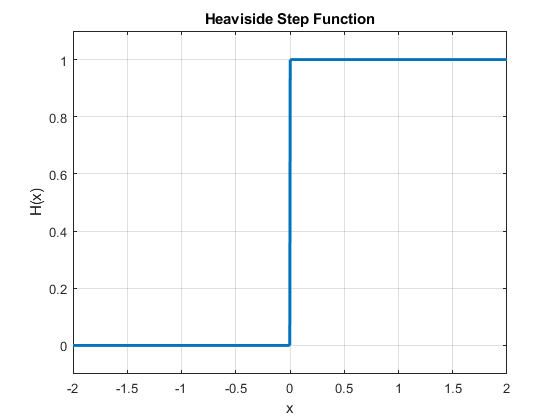
\includegraphics[width=4cm, keepaspectratio]{img/img-ch1/heaviside_graph.png}}\\
        Sigmoid & $\sigma (x) = \frac{1}{1+e^{-x}}$ & \adjustbox{valign=c}{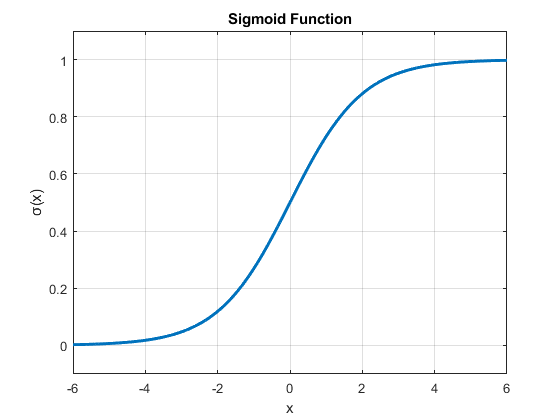
\includegraphics[width=4cm,keepaspectratio]{img/img-ch1/sigmoid.png}} \\
        ReLU & $\sigma(x)=\max\left\lbrace 0, x\right\rbrace $ & \adjustbox{valign=c}{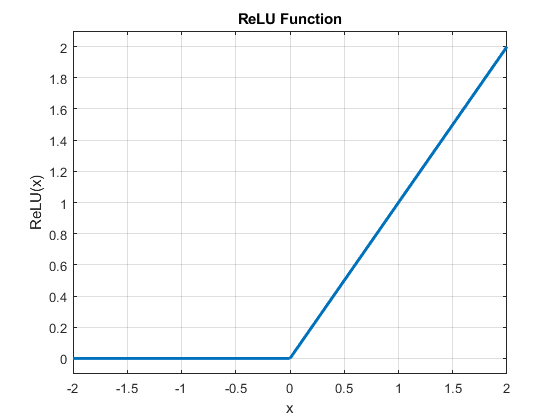
\includegraphics[width=4cm,keepaspectratio]{img/img-ch1/reLU.png}}\\
        Hyperbolic tangent & $\sigma(x)=\tanh (x)$ & \adjustbox{valign=c}{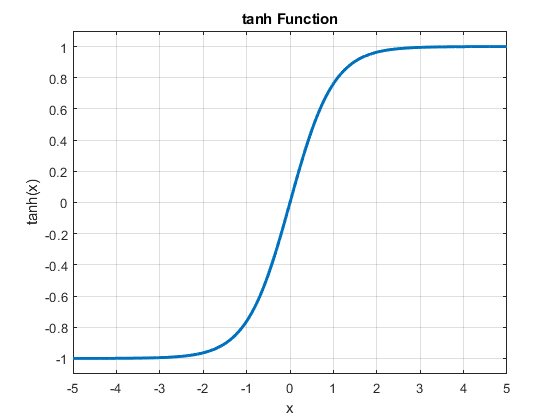
\includegraphics[width=4cm,keepaspectratio]{img/img-ch1/tanh.png}}\\
    \end{tabular}
    \caption{Activation functions}
    \label{tab:activation_functions}
\end{table}

The graphical representation of neural networks (such as \autoref{fig:neural_network}) really helps describing and visualizing its architecture because it intuitively presents information ``flowing'' from the inputs on the far left, along links and through hidden nodes, ultimately to output $f(x)$ on the far right. In order to avoid confusion with the notation, we will make an effort to detail it now that will reward us in the next sections.

Neural networks connect multiple neurons in layers, labeled by $l=0,...,L$ so that the units of each layer are connected to the units of the following layer. In the example of \autoref{fig:neural_network}, $L=3$: the input layer $l=0$, the output layer $l=L$ which determines the value of the function and the layers in between $1 \leq l<L$ are hidden layers. The first layer is formed by input units $x_1,...,x_N$, the following $L-1$ layers contain the hidden neurons $h_{1}^{(l)},...,h_{J_{l}}^{(l)}$ where $l=1,...,L$ and $J_{l}$ is the number of neurons of the $l$-th hidden layer. The last layer consists on the output unit(s). It is common to add a bias term in the weighted sum of the inputs of a neuron, resulting in an extra unit in each layer with fixed value $1$, so that the bias parameter $b$ is taken into account in the computations.

Every arrow represents a weight or connection strength from a neuron in a layer to a neuron in the next layer. The weights are represented by $W_l, \, l=1,...,L$, a real valued matrix of weights of the $l$-th layer. The weight into neuron $j$ in layer $l$ from node $i$ in the previous layer $l-1$ is $w_{l}^{(i \rightarrow j)}$. Each neuron is updated by an activation function depending on all neurons feeding into it, and the update protocol prescribes that each layer is updated after the previous one, thus working layer by layer. When working this way, vector and matrix notation are useful: the output of neurons $1,...,J_l$ in layer $l$ is the vector $X_l \in \left\lbrace 1 \right\rbrace \times \mathbb{R}^{J_l}$ and the matrix of weights $W_l$ of dimension $(J_{l-1}+1) \times J_l$ (taking into account the bias node).

The dimension of each layer $d = [J_{1}, J_{2},..., J_{L}]$ and the number of layers $L$ determines the architecture of the neural network, which means the neural network model family whose parameters will be optimized to choose the specific configuration of weights that best generalises the data.

\begin{figure}
    \centering
    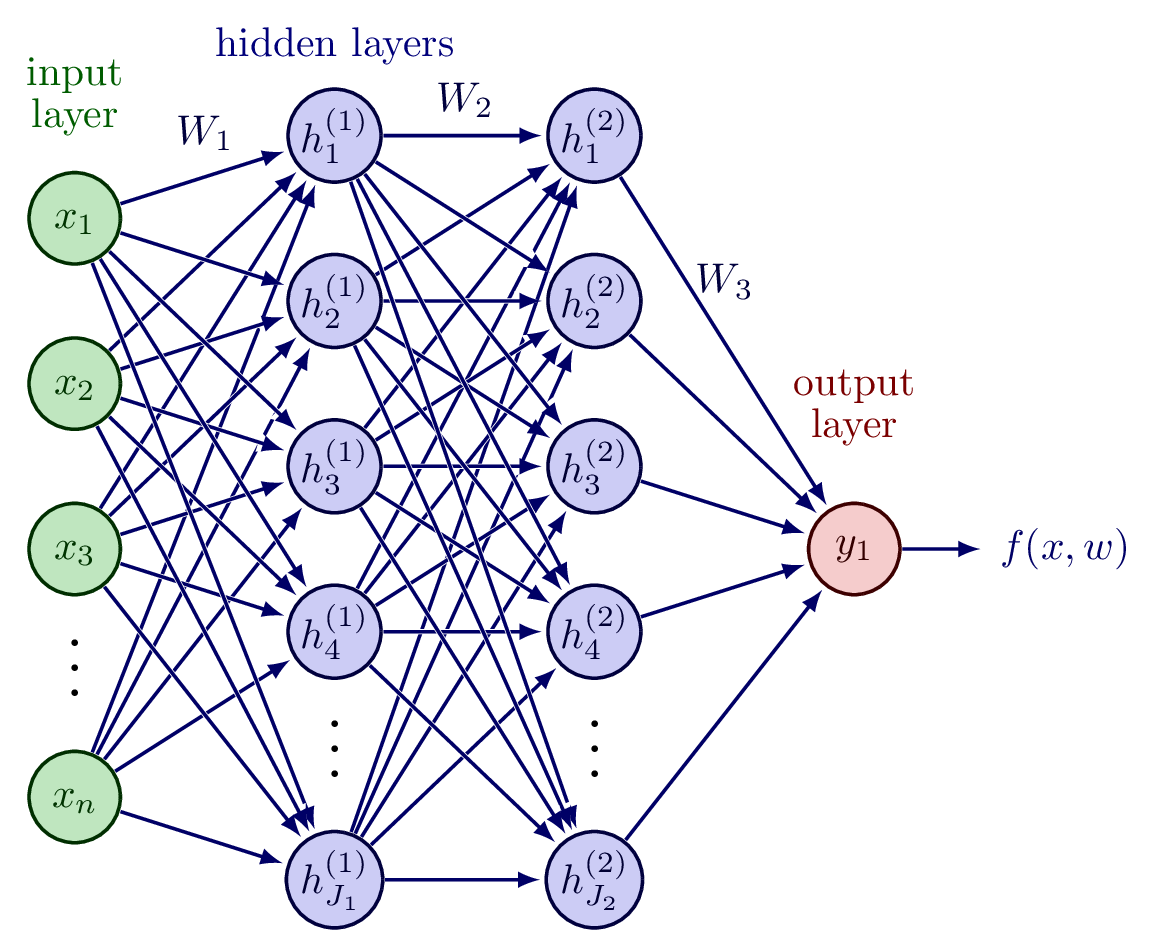
\includegraphics[width=0.8\linewidth]{img/img-ch1/NN.png}
    \caption{Illustration of a neural network. Adapted from \href{https://tikz.net/neural_networks/}{Izaak Neutelings}, \href{https://creativecommons.org/licenses/by-sa/4.0/}{CC BY-SA 4.0}}
    \label{fig:neural_network}
\end{figure}

\subsection{Forward propagation}
The function that expresses the output of a neural network is
\begin{equation}
    f_{W_1, W_2,..., W_L}(x) = \varphi_L(w_L \varphi_{L-1}(W_{L-1} \cdots \varphi_2(W_2 \varphi_1(W_1 x) ) \cdots ) )
\end{equation}
where $x \in\mathcal{X}$, $W_i, \, i=1,...,L$ is a real valued matrix of weights of the $i$-th layer and $\varphi_i$ is the activation function in vectorised form. This is computed by the \textbf{forward propagation algorithm}. Taking into account the bias as node 0, we can observe that the inputs and outputs of a layer are related by
\begin{equation}
    X_l = \begin{bmatrix}
        1 \\
        \sigma(W_l X_{l-1})
    \end{bmatrix} 
\end{equation}
where $\sigma(W_l X_{l-1})$ is a vector whose components are the result of applying the vectorised form of the activation function to the weighted sum (with weights $W_l$) of the outputs from the previous layer ($X_{l-1}$)

This computation starts by initializing the input layer $x_1 = x \in \mathcal{X}$. 

After forward propagation, the output vector $x_l$ at every layer $l=1,...,L$ has been computed. 

\subsection{Backpropagation Algorithm}
Gradient descent is the algorithm used for finding the minimum of a differentiable function. It iteratively updates the parameters $\theta$ of a cost function $C(\theta)$ towards the direction of steepest descent in order to minimize a cost function. In the case of neural networks, the cost function and the model function of the neural network depend on $W = \left\lbrace W_1, ,..., W_L\right\rbrace$. Considering the squared error loss and the dataset $\mathcal{D}=\left\lbrace (x_1,y_1),...,(x_M,y_M)\right\rbrace$, we will work with the following cost function:
\begin{equation}
    C(W)=\frac{1}{M} \sum_{i=1}^M (f(x_i,W)-y_i)^2
\end{equation}

The gradient descent algorithm is our preferred choice for performing the optimisation of the parameters since, when working with nonlinear activation functions, we are facing a difficult optimisation problem that generally is nonlinear and non-convex. The weights are updated in gradient descent at every step $t=1,2,...$ in the following way
\begin{equation}
    W(t+1)=W(t) + \eta \nabla C(W(t))
\end{equation}

To perform gradient descent we need the gradient and to compute the gradient of $C(W)$, we need its derivative with respect to each weight matrix
$$\frac{\partial C}{\partial W_l} = \frac{1}{M}\sum_{i=1}^M \frac{\partial e_n}{\partial W_l}$$
where $e_n=(f(x_n,W)-y_n)^2$

We could think of obtaining $\frac{\partial e}{\partial W_l}$ using the finite differences numerical method. Taking into account we need to compute this method for every weight and for every data point, it becomes computationally prohibitive. The alternative that enables us to compute these gradients is a dynamic programming algorithm known as backpropagation. It is based on several applications of the chain rule. Next, we will deduce the algorithm step by step and then, we will be able to join all the pieces together to write its pseudo-code.

We want to obtain the partial derivative $\frac{\partial e}{\partial W_l}$

First, observe that variations on the weights $W_l$ influence the output $X_L$ of the neural network. We can view schematically this dependency
$$W_l X_{l-1} \stackrel{\sigma}{\longrightarrow} X_l \longrightarrow W_{l+1}X_l \stackrel{\sigma}{\longrightarrow} X_{l+1} \longrightarrow \cdots \longrightarrow X_L = f(x, W) $$
From now on, we will call $W_l X_{l-1}=S_l$, that is, the input of the $l$-th layer. This vector $S_l = [s_{(l),j}]_{j=1}^{J_l}$ corresponds to the inputs of each $j$ node of the $l$-th layer.

Since variations in $W_l$ impact the output $f(x,W)$, in turn, it affects the loss error $e$. Let's view this effect of $W_l$ element-wise. A change in $w_l^{i\rightarrow j}$ only affects $s_{(l),j}$ the input of the $j$-th node of the $l$-th layer because $$s_{(l),j} = \sum_{i=0}^{J_{L-1}}w_l^{i\rightarrow j}x_{(l-1),i}$$
Thus, by the chain rule
\begin{equation}
    \frac{\partial e}{\partial w_l^{i\rightarrow j}} = \frac{\partial s_{(l),j}}{\partial w_l^{i\rightarrow j}} \frac{\partial e}{\partial s_{(l),j}} = x_{(l-1),i} \delta_{(l),j}
\end{equation}
where the last equality follows from the linear relation between $s_{(l),j}$ and $w_l^{i \rightarrow j}$. We have defined $$\delta_{(l),j} = \frac{\partial e}{\partial s_{(l),j}}$$
The vector $$\delta_l = [\delta_{(l),j)}]_{j=1}^{J_l} = \frac{\partial e}{\partial S_{l}}$$ denotes the sensitivity and it quantifies how the error $e$  changes with $S_l$. 

We can obtain $X_{l}$ for every $l=1,...,L$ using forward propagation. So to get the partial derivatives, we need to obtain the sensitivity vectors $\delta_l$ for every layer. It turns out that the sensitivity vectors can be retrieved by ``running backwards'' our neural network. We can explicitly get the sensitivity of the output layer $\delta_L$ because $e=(X_L-y)^2 = (\sigma(S_L)-y)^2$. Therefore,
\begin{align}
    \delta_L &=\frac{\partial e}{\partial S_L} \\
    &= \frac{\partial}{\partial S_L} (X_L -y)^2 \\
    &= 2(X_L-y)\frac{\partial X_L}{\partial S_L} \\
    &= 2(X_L-y)\sigma^\prime(S_L)
\end{align}
is the starting point of the backward recursion.

We will see how to obtain $\delta_{(l),j}$ element-wise. Since $e$ depends on $S_l$ only through $X_l$, by the chain rule
\begin{align}
    \delta_{(l),j} &= \frac{\partial e}{\partial s_{(l),j}} \\
    &= \frac{\partial e}{\partial x_{(l),j}}\frac{\partial x_{(l),j}}{\partial s_{(l),j}} \\
    &= \frac{\partial e}{\partial x_{(l),j}} \sigma^\prime (s_{(l),j})
\end{align}

Next, we will obtain the partial derivative $\frac{\partial e}{\partial X_l}$. A variation in $X_l$ only affects $S_{l+1}$ and thus, $e$. A particular component of $X_l$ can affect every component of $S_{l+1}$, therefore we need to apply the chain rule taking into account all these dependencies:
\begin{align}
    \frac{\partial e}{\partial x_{(l),j}} &= \sum_{k=1}^{J_{l+1}} \frac{\partial s_{(l+1),k}}{\partial x_{(l),j}} \frac{\partial e}{\partial s_{(l+1),k}} \\
    &= \sum_{k=1}^{J_{l+1}} w_{l+1}^{j \rightarrow k} \delta_{(l+1), k}
\end{align}

because
\begin{itemize}
    \item $s_{(l),j} = \sum_{i=0}^{J_{L-1}}w_l^{i\rightarrow j}x_{(l-1),i}$ , 
    then its derivative with respect to $x_{(l-1),j}$ is 
    $$\frac{\partial s_{(l),k}}{\partial x_{(l-1),j}} = w_{l}^{j \rightarrow k}$$

    \item and by definition we have that
    $$\delta_{(l+1),k} = \frac{\partial e}{\partial s_{(l+1),k}} $$
\end{itemize}

Joining it all together, we obtain the expression for the components of the sensitivity vector
\begin{equation}
    \delta_{(l),j} = \sigma^{\prime}(s_{(l),j}) \sum_{k=1}^{J_{l+1}} w_{l+1}^{j\rightarrow k} \delta_{(l+1),k}
\end{equation}
This resulting equation to compute the sensitivity at the $l$-th layer is expressed in terms of the sensitivity in the next layer $l+1$, producing a backward recursion. Therefore, if we know the sensitivities at layer $l+1$, we can get $\delta_l$. 

The consequent vector expression of the sensitivity is
\begin{equation}
    \delta_l = \sigma^{\prime}(S_l) \odot [(W_{l+1})^T\delta_{l+1}]_{1}^{J_l}
\end{equation}
where $\odot$ denotes the Hadamard product, the elementwise product of the two vectors: \\ $u,v \in \mathbb{R}^n$, then $u \odot v $ is a vector such that $ (u \odot v)_i =u_i v_i, \, i = 1,...,n$. 

In the vector equation of the sensitivity $\delta_l$ in terms of the sensitivity in the next layer $\delta_{l+1}$, $W_{l+1}$ is the transpose of the weight matrix of the $l+1$-th layer, $W_{l+1}$. When we apply this transpose weight matrix we can think intuitively as moving the sensitivity error backward through the network. Then, we can interpretate the Hadamard product of $\sigma^{\prime}(S_l)$ as moving the sensitivity error backwards through the activation function in layer $l$. 

\begin{tcolorbox}[title=Backpropagation algorithm]
    \textbf{Input:} a data point $(X,y)$
    \begin{enumerate}
        \item Run forward propagation on $X$ to compute and save $X_l$ and $S_l$ for $l=1,...,L$

        \item \textbf{Initialization} 
        
        $\delta_L \leftarrow 2(X_L - y)\sigma^{\prime}(S_L)$

        \item \textbf{Backpropagation recursion}

        for $l=L-1$ to $1$ do:
        
        \qquad $\delta_l \leftarrow \sigma^{\prime}(S_l) \odot [(W_{l+1})^T\delta_{l+1}]_{1}^{J_l}$
    \end{enumerate}
    
\end{tcolorbox}


Finally, as a recapitulation, we will remember our goal was to perform gradient descent to optimise the weights of the neural network, for which we needed the gradient of the cost function with respect to every weight parameter. Using the chain rule, the expression for the required partial derivatives is
\begin{equation}
    \frac{\partial e}{\partial w_l^{i\rightarrow j}} = x_{(l-1),i} \delta_{(l),j}
\end{equation}

We can compute it because we can obtain the term $X_l,\, l=1,...,L$ with the forward propagation recursion
\begin{equation}
    X_l = \begin{bmatrix}
        1 \\
        \sigma(W_l X_{l-1})
    \end{bmatrix} 
\end{equation}
with initial condition $X_0=X\in \mathcal{X}$, the input vector.

On the other hand, we can calculate the sensitivities $\delta_l, \, l=1,...,L$ with backpropagation using the recursion 
\begin{equation}
    \delta_l = \sigma^{\prime}(S_l) \odot [(W_{l+1})^T\delta_{l+1}]_{1}^{J_l}
\end{equation}
with initial condition $\delta_L = 2(X_L - y)\sigma^{\prime}(S_L)$.



\endinput
%--------------------------------------------------------------------
% FIN DEL CAPÍTULO. 
%--------------------------------------------------------------------
